\chapter{System Design and Methodology}
\section{AR4 Restoration and Hardware Modifications}
The AR4 robotic manipulator was handed over to the current
team by the previous graduation project team after their completion of the project.
At the time of handover, the robot was delivered in a fully assembled
condition and was generally operational. The unit is an AR4 MK3 model designed by
Chris Annin. However, due to the duration and intensity of prior
usage during development and testing, several components exhibited
wear and assembly-related issues. As a result, multiple mechanical
and electrical corrective actions were required before the 
robot could be considered reliable for accurate motion execution and 
experimental work.
\subsection{Joint 3 Mechanical Transmission Upgrade}
Joint~3 of the AR4 robot exhibited significant backlash due 
to wear and limitations in the original mechanical transmission 
design. To address this issue, the joint transmission system was 
completely replaced in accordance with the official upgrade 
provided by Chris Annin. The upgrade consisted of a redesigned 
gear set and a new timing belt, both intended to improve torque 
transmission and reduce mechanical play within the joint.

\begin{figure}[H]
    \centering
    % 
\includegraphics[width=0.75\textwidth]{figures/AR4 modifications/Joint3_mods.png}
    \caption{Upgraded mechanical transmission of Joint~3 }
    \label{fig:joint3_upgrade}
\end{figure}

After implementing the upgraded components, the backlash in 
Joint~3 was reduced from approximately $6^\circ$ to $3^\circ$. 
This reduction resulted in smoother joint motion and improved 
positioning accuracy, directly enhancing the overall kinematic 
performance of the robot.

\subsection{Shaft Key Re-Manufacturing in Joint 3}
Despite the improvements achieved through the mechanical 
transmission upgrade, residual backlash was still observed in 
Joint~3. Further investigation revealed that the shaft key 
responsible for transmitting motion from the second gear stage 
to the robotic arm link exhibited wear and improper fit. 
This condition introduced mechanical play within the joint, 
negatively affecting positioning accuracy.

\begin{figure}[H]
    \centering
    % 
\includegraphics[width=0.45\textwidth, angle=90]{figures/AR4 modifications/Shaft_key.png}
    \caption{Re-manufactured shaft key used in Joint~3 to eliminate mechanical backlash}
    \label{fig:shaft_key}
\end{figure}

To resolve this issue, the shaft key was re-manufactured with 
precise dimensions to ensure a tight and accurate fit between 
the gear and the arm shaft using hot-wire machining. The newly manufactured key eliminated 
relative motion between the connected components, effectively 
removing the remaining backlash in Joint~3. As a result, 
Joint~3 achieved backlash-free motion, significantly improving 
the repeatability and accuracy of the robot during operation.

\subsection{Encoder Signal Noise in Joints 5 and 6}

During system testing and motion execution, unstable and noisy encoder readings were observed in Joints~5 and~6 of the AR4 robot. These fluctuations resulted in inaccurate joint position feedback, which significantly affected the forward and inverse kinematics calculations. Consequently, commanded joint positions did not always correspond to the expected physical motion of the robot.

A systematic debugging process was conducted, including signal tracing and verification of the encoder wiring and power connections. This investigation revealed that the encoders of Joints~5 and~6 were not properly connected to the regulated $5\,\text{V}$ power supply. The improper power connection caused voltage instability, leading to fluctuating encoder signals and unreliable position measurements.

After correcting the power supply connections and ensuring proper grounding, the encoder signals became stable and consistent. This correction restored accurate joint position feedback, significantly improving the reliability of the kinematic calculations and overall motion control performance of the robot.


\section{Cartesian Calibration of the AR4 Collaborative Robot}

\thispagestyle{fancy}
\vspace*{0cm} % move text up to start near top of page
\label{sec:ar4_calibration}

Accurate positioning is critical in collaborative robotic applications, particularly when multiple manipulators operate within a shared workspace. During initial experimental trials, the AR4 robotic arm exhibited noticeable Cartesian positioning inaccuracies when executing commanded end-effector positions relative to the ABB robot world coordinate frame. These inaccuracies motivated the implementation of a dedicated Cartesian calibration procedure to improve the absolute positioning accuracy of the AR4 robot.

\subsection{Experimental Setup}

The calibration experiment was conducted using a pointed end-effector mounted on the AR4 robot to enable precise position referencing. A calibrated measurement grid with millimeter resolution was placed on the worktable. The grid origin was aligned with the ABB robot world frame origin $(0,0,0)$, ensuring a common global reference for both manipulators.

The AR4 robot was commanded to move to a predefined set of Cartesian positions distributed over the XY plane at multiple height levels along the Z-axis. At each commanded position $(x_{cmd}, y_{cmd}, z_{cmd})$, the actual end-effector position $(x_{meas}, y_{meas}, z_{meas})$ was manually recorded using the grid.

\subsection{Cartesian Error Characterization}

The raw Cartesian positioning errors were computed as:
\begin{equation}
\begin{aligned}
e_x &= x_{meas} - x_{cmd} \\
e_y &= y_{meas} - y_{cmd} \\
e_z &= z_{meas} - z_{cmd}
\end{aligned}
\end{equation}

Initial analysis revealed systematic and spatially correlated errors across the workspace, indicating that the inaccuracies were not purely random but instead dependent on the commanded Cartesian position.

\subsection{Calibration Method Selection}

Several calibration approaches were evaluated prior to selecting the final method. Table~\ref{tab:calib_comparison} summarizes the comparison between candidate techniques. The calibration dataset was divided into independent training and testing subsets to ensure that the reported performance reflects generalization rather than overfitting to the calibration points.

\begin{table}[H]
\centering
\renewcommand{\arraystretch}{1.3}
\begin{tabular}{|c|c|c|c|c|}
\hline
\textbf{Method} &
\textbf{Accuracy} &
\textbf{Extrapolation} &
\textbf{Data Requirements} &
\textbf{Real-Time} \\ \hline

Lookup
Table &
Medium &
None &
High &
High \\ \hline

RBF
Network &
High &
Poor &
Very High &
Medium \\ \hline

Spline
Fitting &
High &
Limited &
Medium &
High \\ \hline

Polynomial
Regression &
High &
Good (Low-Order) &
Medium &
High \\ \hline

\end{tabular}
\caption{Comparison of Cartesian calibration methods for robotic manipulators}
\label{tab:calib_comparison}
\end{table}

Based on this comparison, the polynomial calibration was selected as a balanced solution, offering a favorable trade-off between accuracy, robustness, and implementation simplicity, making it particularly suitable for real-time correction in collaborative robotic systems.

\subsection{Polynomial Calibration Model}

A second-order polynomial regression model was used to approximate the Cartesian error as a function of the commanded XY position:
\begin{equation}
e(x,y) = a_1 x + a_2 y + a_3 x^2 + a_4 y^2 + a_5 xy + a_6
\end{equation}

The estimated polynomial error models were used to correct the commanded positions prior to execution:
\begin{equation}
\begin{aligned}
x_{corr} &= x_{cmd} + \hat{e}_x(x,y) \\
y_{corr} &= y_{cmd} + \hat{e}_y(x,y) \\
z_{corr} &= z_{cmd} + \hat{e}_z(x,y)
\end{aligned}
\end{equation}

This correction strategy enables feedforward compensation of systematic positioning errors without modifying the internal robot controller.

\subsection{Calibration Results}

Based on the experimental results, all evaluated calibration approaches significantly reduced the Cartesian positioning error when compared to the uncalibrated model. Among the tested methods, the linear model exhibited the highest residual error due to its inability to capture nonlinear kinematic and geometric effects. Radial Basis Function (RBF) networks achieved the lowest mean positioning error, demonstrating superior interpolation accuracy within the calibrated workspace. However, their locally adaptive nature resulted in less predictable behavior near the workspace boundaries and outside the training region. \\

The second-degree polynomial model produced slightly higher errors than the RBF-based approach, yet these errors remained within acceptable limits for the intended application. In contrast to RBF and spline-based methods, the polynomial model exhibited smoother and more stable behavior near workspace boundaries, while maintaining low computational cost and consistent real-time performance. \\

Figure~\ref{fig:xy_error_before} illustrates a comparison between the commanded, measured, and polynomial-corrected end-effector positions in the XY plane. The deviation between the commanded and measured positions highlights the presence of systematic Cartesian positioning errors in the AR4 robot, while the corrected positions demonstrate the effectiveness of the polynomial calibration in compensating for these errors.

\begin{figure}[H]
    \centering
    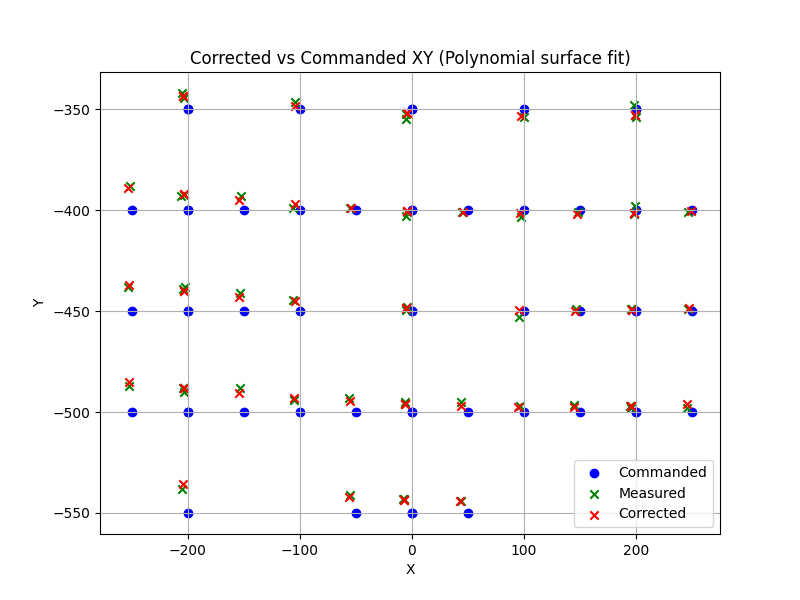
\includegraphics[width=0.8\textwidth]{Figures/Calibration/Poly_corrections.png}
    \caption{XY-plane commanded, measured, and corrected positions.}
    \label{fig:xy_error_before}
\end{figure}

\subsection{Error Surface Analysis}

To further analyze the spatial behavior of the calibration model, three-dimensional polynomial error surfaces were generated for each Cartesian axis, which are shown in Figure~\ref{fig:poly_error_surfaces}

\begin{figure}[H]
    \centering
    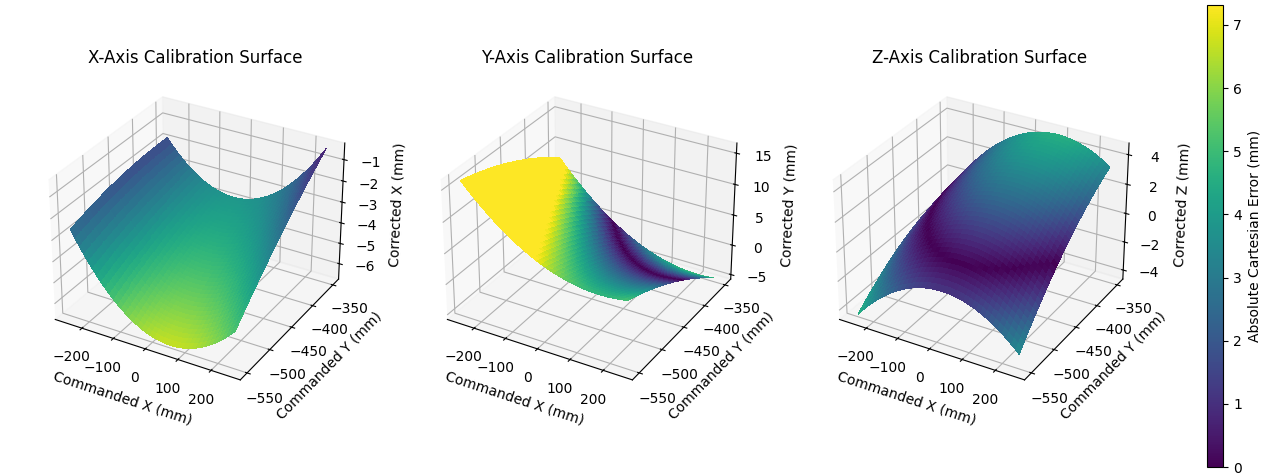
\includegraphics[width=\textwidth]{Figures/Calibration/Poly_3D.png}
    \caption{Calibration surfaces for the X, Y, and Z axes with error magnitude.}
    \label{fig:poly_error_surfaces}
\end{figure}

Figure~\ref{fig:calibrated_vs_uncalibrated_surface} presents a comparison between the uncalibrated and calibrated surfaces.The comparison demonstrates that the calibration model effectively smooths and compensates for the dominant systematic error components, resulting in a more uniform and stable error distribution across the workspace.

\begin{figure}[H]
    \centering
    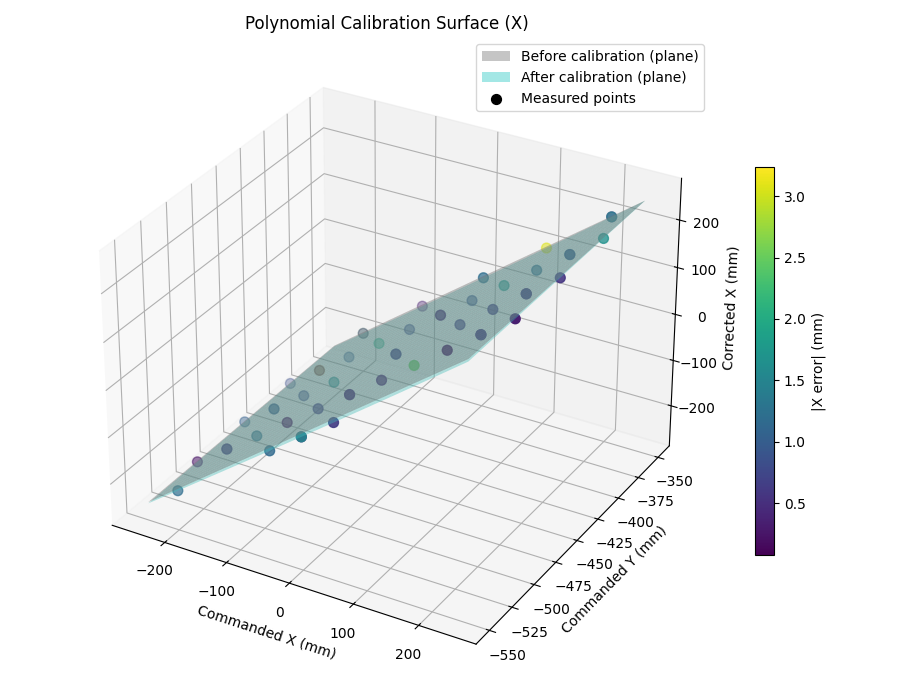
\includegraphics[width=0.47\textwidth]{Figures/Calibration/Poly_X.png}
    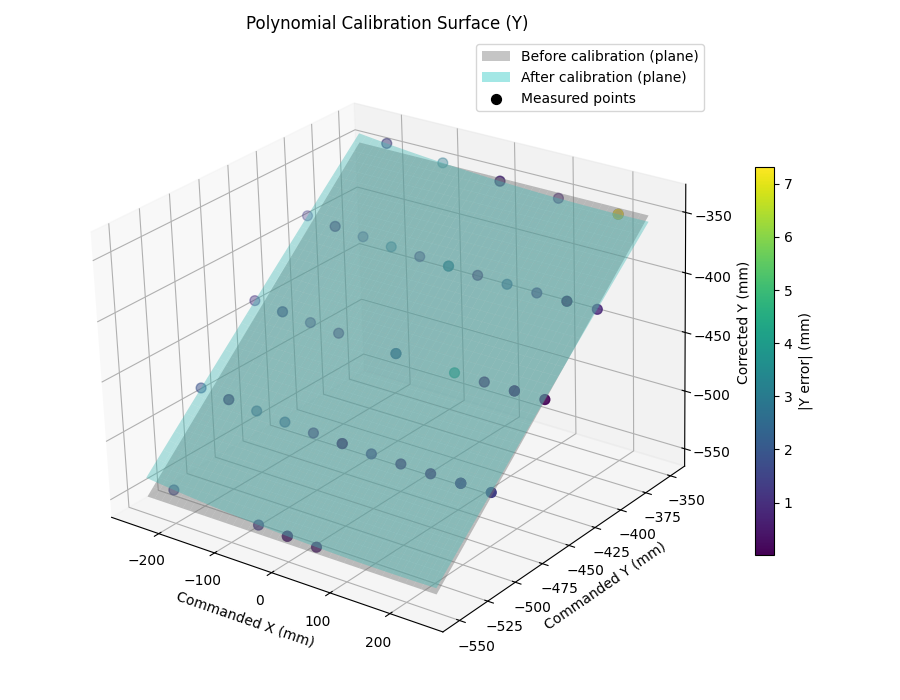
\includegraphics[width=0.47\textwidth]{Figures/Calibration/Poly_Y.png}
    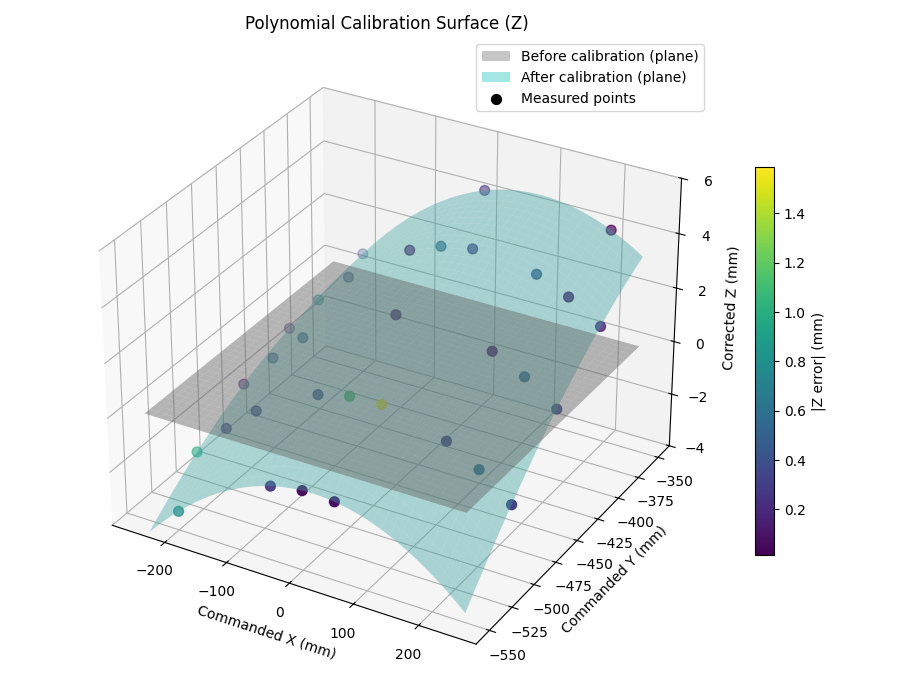
\includegraphics[width=0.47\textwidth]{Figures/Calibration/Poly_Z.png}
    \caption{Comparison of uncalibrated and calibrated surfaces.}
    \label{fig:calibrated_vs_uncalibrated_surface}
\end{figure}

% \begin{figure}[h]
%     \centering
%     \begin{subfigure}{0.32\textwidth}
%         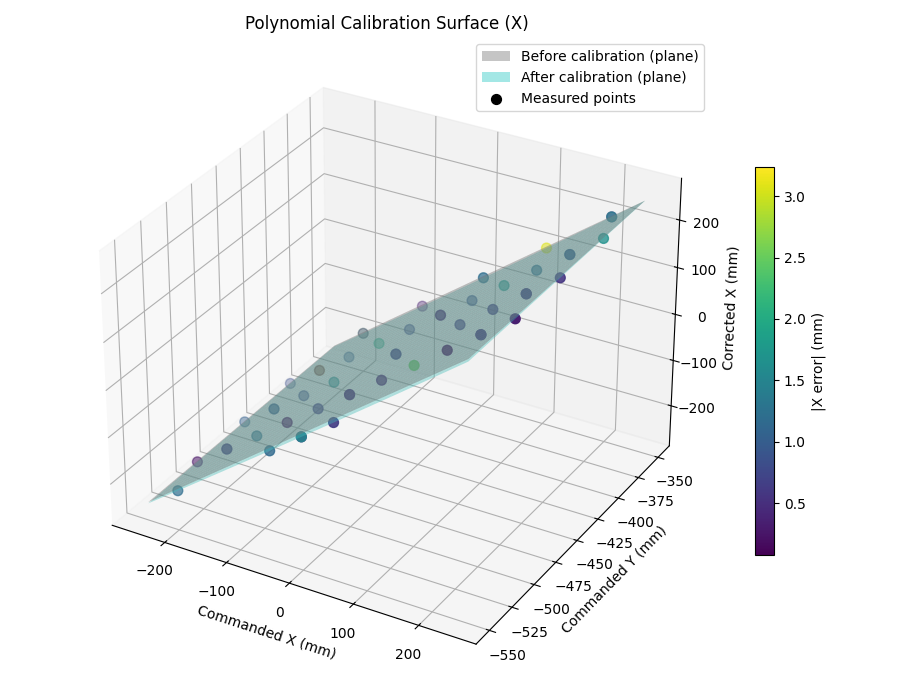
\includegraphics[width=\linewidth]{Figures/Calibration/Poly_X.png}
%     \end{subfigure}
%     \hfill
%     \begin{subfigure}{0.32\textwidth}
%         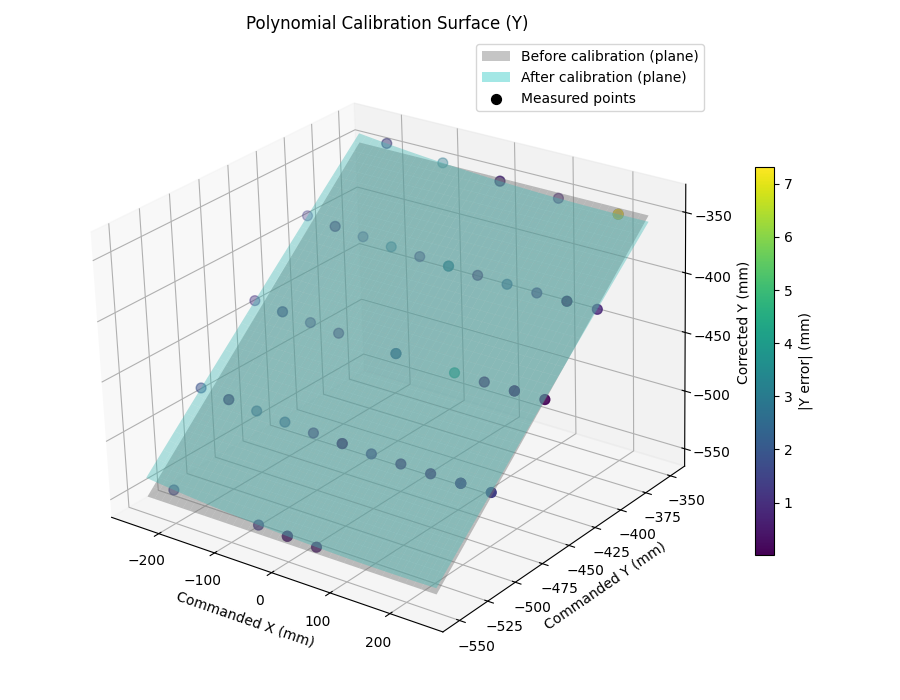
\includegraphics[width=\linewidth]{Figures/Calibration/Poly_Y.png}
%     \end{subfigure}
%     \hfill
%     \begin{subfigure}{0.32\textwidth}
%         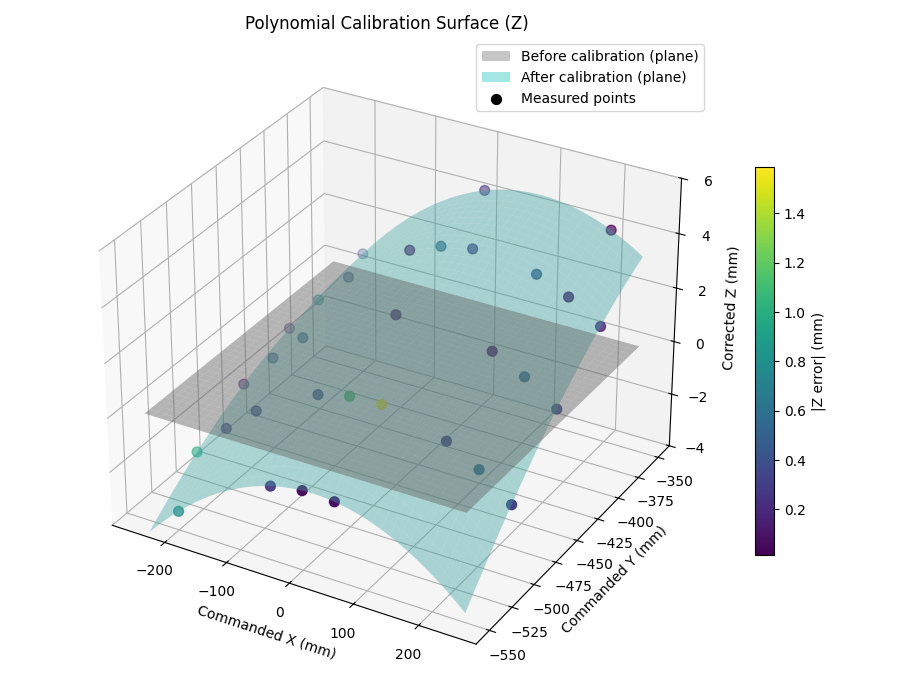
\includegraphics[width=\linewidth]{Figures/Calibration/Poly_Z.png}
%     \end{subfigure}

%     \caption{Polynomial calibration error surfaces for the X, Y, and Z Cartesian axes.}
%     \label{fig:poly_surfaces}
% \end{figure}

\subsection{Quantitative Evaluation}


The effectiveness of the calibration was quantitatively evaluated using the mean absolute error (MAE) before and after correction for each Cartesian axis, computed on the independent test dataset.

\begin{table}[H]
\centering
\caption{Mean Absolute Cartesian Errors Before and After Calibration}
\label{tab:mae_results}
\renewcommand{\arraystretch}{1.2}
\begin{tabular}{|c|c|c|}
\hline
\textbf{Axis} & \textbf{MAE Before (mm)} & \textbf{MAE After (mm)} \\ \hline
X & 3.96 & 0.94 \\ \hline
Y & 5.13 & 1.32 \\ \hline
Z & 1.94 & 0.46 \\ \hline
\end{tabular}
\end{table}

The quantitative results in Table~\ref{tab:mae_results} are consistent with the smooth and continuous behavior observed in the polynomial error surfaces shown in Figure~\ref{fig:poly_error_surfaces}, confirming the effectiveness and stability of the proposed calibration approach.
